% Leave unused column space at the bottom instead of stretching paragraphs.
\documentclass[reprint,aps,pra,amsmath,amssymb,floatfix,raggedbottom]{revtex4-2}
\usepackage{graphicx}
\usepackage{booktabs}
\usepackage{hyperref}
\hypersetup{colorlinks=true,linkcolor=blue,citecolor=blue,urlcolor=blue}
\graphicspath{{reports/figures/}{figures/}}
\newcommand{\mjj}{m_{JJ}}
\newcommand{\AUC}{\mathrm{AUC}}
\begin{document}
\title{Benchmarking unsupervised and semi-supervised anomaly detection on the LHC Olympics 2020 R\&D dataset}
\author{Mithil Hardik Astik}
\email{f20240923@hyderabad.bits-pilani.ac.in}
\affiliation{Department of Physics, BITS Pilani, Hyderabad Campus, Hyderabad, Telangana, India}
\date{October 3, 2026}
\begin{abstract}
Model-agnostic searches for new physics at the Large Hadron Collider seek departures from the dominant quantum chromodynamics background without fixing a single signal hypothesis. We benchmark unsupervised, semi-supervised, and supervised detectors on the simulated LHC Olympics 2020 research and development dataset, examining label efficiency, training contamination, mass sculpting, and topology transfer. A shared event split and five standardized jet observables support 47 core fits, including five-seed comparisons of six headline configurations. Isolation Forest reaches nominal area under the receiver operating characteristic curve $0.8068\pm0.0077$; Deep SAD with 100 known anomalies and 0.5\% unlabelled training contamination reaches $0.8880\pm0.0114$. These uncertainties describe training-seed dispersion, while paired bootstrapping separately quantifies finite-test uncertainty. Deep SAD retains area $0.7492\pm0.0614$ on a held-out three-prong topology, compared with $0.9292\pm0.0012$ for the fully supervised reference. Background mass diagnostics reveal that strong ranking and stable search-variable distributions are distinct requirements. An approximate sideband-fit study, archived particle and density extensions, and an unevaluated mass-decorrelated candidate identify the remaining validation questions. The results provide a reproducible classical benchmark with explicit implementation and statistical limitations, rather than a calibrated discovery claim.
\end{abstract}
\maketitle

\section{Introduction}
Searches for new particles often specify a signal model before defining discriminating observables. Anomaly detection instead attempts to identify departures from a reference distribution, potentially retaining sensitivity to signals outside a narrowly chosen training hypothesis. The LHC Olympics challenge established a public setting for assessing such approaches and demonstrated the variety of available supervision strategies \cite{lhco}. This motivation does not remove the need for an explicit reference distribution, an evaluation protocol, or a statistical model for a claimed excess.

The motivation is also experimental: ATLAS has performed a weakly supervised dijet-resonance search, and CMS has used complementary unsupervised, weakly supervised, and semi-supervised anomaly selections in collision data \cite{atlas,cms}. These searches establish the relevance of the problem, while emphasizing the distinction between a simulation benchmark and an analysis with detector uncertainties and background controls. Here ``model-agnostic'' refers to reduced dependence on a prescribed signal template; the choice of observables, reference events, score, and resonance window still supplies physical assumptions.

Reconstruction errors, isolation-based scores, and compact learned representations encode different assumptions about unusual events. Deep SVDD learns a representation concentrated about a fixed center \cite{svdd}; Deep SAD extends that principle using known anomalous examples \cite{sad}. Collider applications also include weakly supervised signal-region classifiers \cite{cwola}, conditional density ratios \cite{anode}, and classification against generated reference events \cite{cathode}. Consequently, neither limited supervision nor a combination of anomaly ranking and a resonance search is intrinsically a new method.

This study focuses on four practical questions. How robust are unsupervised detectors to unlabelled signal contamination? How much discrimination can a small labelled-anomaly budget provide? What distortion of the dijet-mass spectrum accompanies the score selection? And how much of the ranking transfers to a structurally different signal topology? We address these questions within one fixed feature representation, reporting negative outcomes as well as successful rankings and distinguishing training variability from uncertainty in the finite evaluation sample.

The principal contribution is the common protocol, released checkpoints and scores, and an implementation audit that makes the comparison reproducible. It is not a claim of state-of-the-art performance: the published density-estimation methods are not reproduced faithfully by the exploratory proxies, and a physics-motivated subjettiness cut remains an important reference. All numerical conclusions below refer to simulated samples and the stated observables, rather than detector data or an unrestricted family of possible signals.

The detector catalog retains the original study's M0--M12 organization, but separates repeatedly evaluated core models, archived single-seed comparisons, and the mass-decorrelated candidates whose performance remains unvalidated. This distinction allows the broader research program to be described without presenting every implemented idea as an established result. The central methodological lesson is to report discrimination jointly with label cost, robustness to contamination, topology dependence, and mass-spectrum stability.

\section{Dataset and experimental protocol}
\subsection{Samples, observables, and units}
The official research and development sample contains one million quantum chromodynamics background events and 100,000 nominal signal events. The nominal process is $W'\to XY$ with $X,Y\to q\bar q$, masses $m_{W'}=3.5$ TeV, $m_X=500$ GeV, and $m_Y=100$ GeV. An additional 100,000-event sample changes the daughter decays to three-prong jets. The data were generated with Pythia and Delphes, without pileup or multiple parton interactions, and use an anti-$k_T$ jet definition with radius one and a leading-jet trigger threshold of 1.2 TeV \cite{dataset,lhco}. These are properties of the supplied simulation, not generation choices newly studied here.

We use the supplied high-level jet observables rather than claim an independent reconstruction of their complete clustering and subjettiness configuration. The mass-blind input vector is
\begin{equation}
 x=(m_{J_1},|m_{J_1}-m_{J_2}|,\tau_{21}^{J_1},\tau_{21}^{J_2},\Delta R_{JJ}),
\end{equation}
where $\tau_{21}=\tau_2/\tau_1$ is a subjettiness ratio \cite{tau}. The dijet invariant mass $\mjj$ is retained for diagnostics and the sideband study; it is also supplied to the mass-aware reference as a sixth feature. We use the high-energy convention $c=1$: masses and momenta are quoted in GeV or TeV, while angular distances and subjettiness ratios are dimensionless. Standardized network inputs and anomaly scores are dimensionless.

\begin{table}[tbp]
\caption{Canonical five-feature representation before standardization. $J_1$ and $J_2$ denote the leading and subleading jets. The absolute mass difference has units of mass; it is not a normalized asymmetry.}\label{tab:features}
\begin{ruledtabular}\begin{tabular}{cll}
Index & Observable & Units\\
0 & $m_{J_1}$ & GeV\\
1 & $|m_{J_1}-m_{J_2}|$ & GeV\\
2 & $\tau_{21}^{J_1}$ & Dimensionless\\
3 & $\tau_{21}^{J_2}$ & Dimensionless\\
4 & $\Delta R_{JJ}$ & Dimensionless
\end{tabular}\end{ruledtabular}
\end{table}

Removing nonfinite or invalid high-level rows excludes 107 events from the combined nominal sample and 25 from the three-prong sample. The retained counts are shown in Table~\ref{tab:split}. The three-prong events are reserved for evaluation throughout the core comparison. This topology-transfer test shares simulation assumptions and resonance masses with the nominal hypothesis; it is not a generator-systematics or mass-extrapolation test.

\begin{table}[tbp]
\caption{Fixed core split after high-level feature validity checks. The three-prong sample is an independent evaluation pool.}\label{tab:split}
\begin{ruledtabular}\begin{tabular}{lrrr}
Sample & Training & Validation & Test\\
Background & 599952 & 199984 & 199984\\
Two-prong signal & 59983 & 19994 & 19996\\
Three-prong signal & 0 & 0 & 99975
\end{tabular}\end{ruledtabular}
\end{table}

\subsection{Separation of training, validation, and test information}
A class-stratified 60/20/20 split is generated with seed 42 and reused across configurations. Subsequent training seeds change initialization, ordering, and signal sampling, but do not create independent test datasets. For the autoencoder, Isolation Forest, Deep SVDD, Deep SAD, and mass-aware reference, feature means and standard deviations are fitted on training background only. The fully supervised reference instead fits its scaler on all nominal training events. Both procedures exclude validation and test events; the preprocessing difference nevertheless prevents attributing the entire supervised advantage to labels alone.

We define the contamination configuration $f$ in percent relative to the training-background count, and inject
\begin{equation}
 n_{\mathrm{inj}}=\left\lfloor {f\over100}N_{B,\mathrm{train}}\right\rfloor
\end{equation}
nominal signal events into the unlabelled training pool. Thus $f=0.5$ means 0.5\%, not 50\%. Deep SAD additionally receives $k$ known anomalies drawn without overlap with the injected unlabelled signal events. The headline $f=0.5$, $k=100$ configuration contains 2,999 unlabelled signal events. Labels for the test pools never enter detector optimization.

The fully supervised network uses all 59,983 training signal labels. Its configuration name contains a $k=1000$ field, but that field is metadata and does not restrict its training labels. We therefore describe this model as a fully supervised reference, not as a 1,000-label competitor. Supervised validation also uses both classes; the other neural models select checkpoints using a background validation objective.

\subsection{Configuration coverage}
At seed 42, the core grid contains four contamination settings $f\in\{0,0.1,0.5,1\}$ for each of the three unsupervised methods, nine Deep SAD settings from $f\in\{0,0.5,1\}$ and $k\in\{10,100,1000\}$, and two reference configurations. Six headline configurations are repeated at seeds 43--46, giving 47 fits in total. Five-seed results therefore apply to the headline settings, not to every point in the contamination or label-budget grid. The canonical results table also retains five separately identified exploratory high-level configurations.

These settings were examined on a public, previously studied signal. The release tag freezes artifacts for reproducibility; it does not turn a retrospective comparison into a prospectively blinded discovery experiment. There is no statistically independent validation of a configuration chosen using its reported test AUC.

\section{Detectors and optimization}
\subsection{Unsupervised baselines}
The autoencoder has widths $5\to64\to32\to16\to32\to64\to5$, biased linear layers, and LeakyReLU activations. Its training loss and score are the mean squared reconstruction error,
\begin{equation}
 L_{\mathrm{AE}}={1\over5|U|}\sum_{i\in U}\|x_i-\hat x_i\|_2^2,
 \qquad s_{\mathrm{AE}}(x)={\|x-\hat x\|_2^2\over5}.
\end{equation}
An error measures incompatibility with this learned reconstruction, not a calibrated likelihood ratio. This distinction is relevant to collider autoencoder searches \cite{autoencoder}.

Isolation Forest uses 100 trees, automatic contamination and subsampling settings (256 events per tree in the employed implementation), and a seed-specific random state. Higher anomaly scores are obtained by negating the decision function. The construction is the existing isolation-based algorithm \cite{iforest}; it has no neural trainable-parameter count comparable to those below.

The Deep SVDD embedding has bias-free widths $5\to64\to32\to16$ and ReLU hidden activations. Let $q_i=\|\phi_\theta(x_i)-c\|_2^2$. Its objective is the minibatch mean of $q_i$. The center $c$ is initialized from the mean embedding of the initial unlabelled pool and then fixed; small nonzero components are clamped to magnitude 0.1, whereas exact zeros remain zero. No autoencoder pretraining is used. In contaminated configurations the initialization pool includes the injected signal. These implementation choices matter when interpreting a near-chance outcome; that outcome alone does not establish representation collapse.

\subsection{Limited supervision and references}
Deep SAD uses the same embedding and center prescription. With unlabelled and known-anomalous subsets $U_b,A_b$ in batch $b$, the implementation minimizes
\begin{equation}\label{eq:sad}
 L_b={1\over|U_b|}\sum_{i\in U_b}q_i+
 {\eta\over|A_b|}\sum_{j\in A_b}{1\over q_j+\epsilon},
\end{equation}
where $\eta=1$ and $\epsilon=10^{-6}$. The second term is omitted for a batch containing no labelled anomaly. The terms encourage small distances for the unlabelled reference and large distances for known anomalies. This is an implementation of the established Deep SAD principle \cite{sad}, with separately averaged batch terms. It is not a uniformly weighted global loss over all samples. Labelled examples are mixed into the ordinary batch sampler without oversampling, so their frequency and the batch composition change the effective training dynamics as $k$ changes. Early stopping uses background distance alone rather than Eq.~\eqref{eq:sad} on a labelled validation pool.

The supervised reference has widths $5\to64\to32\to1$, biased layers, ReLU hidden activations, and binary cross-entropy with logits. Its sigmoid output is the anomaly score. The mass-aware reference replaces the SVDD input width by six and otherwise uses the same training prescription. This tests explicit mass inclusion in that particular hypersphere architecture, not in every anomaly detector.

Neural models use Adam with learning rate $10^{-3}$, weight decay $10^{-5}$, batch size 256, at most 50 epochs, and early-stopping patience eight. Parameter counts are 5,973 for the autoencoder, 2,880 for each five-feature hypersphere network, 2,497 for the supervised reference, and 2,944 for the mass-aware model. Capacities and validation objectives are not identical across methods; this is a comparison of specified practical implementations rather than an architecture-matched causal experiment.

\section{Evaluation and uncertainty}
\subsection{Ranking and topology transfer}
For a score increasing with anomalousness, the empirical AUC estimates
\begin{equation}
 \Pr[s(X_S)>s(X_B)]+\tfrac12\Pr[s(X_S)=s(X_B)].
\end{equation}
The nominal test pool contains 199,984 background and 19,996 signal events, a signal prevalence of 9.0899\%. This deliberate evaluation mixture is distinct from the much smaller training injection. AUC is a ranking statistic and does not imply the same precision, discovery reach, or background rate at arbitrary physical signal prevalence.

We also inspect background rejection at specified signal efficiencies and the significance-improvement characteristic $\epsilon_S/\sqrt{\epsilon_B}$ on ROC points with $\epsilon_B>0$. This expression describes the background-dominated counting approximation; it is not a replacement for a nuisance-aware likelihood or a measure at a finite zero-background tail. ROC-selected test thresholds are descriptive only. Topology transfer is assessed using the same frozen detector score on the three-prong pool and the shared background test events.

For five-seed results we report the arithmetic mean and sample standard deviation, not a standard error or confidence interval. Separately, 500 stratified paired bootstrap resamples of the frozen seed-42 test scores use seed 20261003. Each resample preserves the class sample sizes, uses common event multiplicities across models, and handles tied scores with half credit. Percentile 95\% intervals condition on the already trained detector and shared test distribution. They do not include optimization uncertainty, detector systematics, or uncertainty caused by choosing a model after inspecting the test results.

\subsection{Mass sculpting and calibrated score cuts}
Cuts intended to retain 10\% or 1\% of background are calibrated on validation background and frozen before test evaluation. Ties are accepted fractionally to attain the intended validation efficiency in expectation. The resulting weighted counts represent randomized acceptance probabilities; they are not necessarily integer event counts.

We quantify background mass changes through the Jensen--Shannon divergence
\begin{equation}
\begin{aligned} J(P,Q)&=\tfrac12D_{\mathrm{KL}}(P\|M)+\tfrac12D_{\mathrm{KL}}(Q\|M),\\
 M&=\tfrac12(P+Q).\end{aligned}
\end{equation}
using natural logarithms and normalized histograms with 49 equal-width bins between 2 and 5 TeV. Here $P$ is the inclusive test-background mass histogram and $Q$ is the selected histogram. We also record Pearson correlation between score and mass. Low binned divergence or low linear correlation does not establish conditional independence, nor rule out a localized feature that compromises a resonance search.

\subsection{Approximate local-excess diagnostic}
The sideband study fits 40 bins between 2.5 and 4.5 TeV, each 50 GeV wide, excluding the fixed signal window 3.3--3.7 TeV. With $x=\mjj/(13000\,\mathrm{GeV})$, the expected bin counts follow
\begin{equation}\label{eq:shape}
 \ln\lambda(x)=a+b\ln(1-x)-c\ln x-d(\ln x)^2.
\end{equation}
Thus logarithms have dimensionless arguments and $\lambda$ denotes a count per fixed bin. Sideband Poisson fits use bounded optimization and the background yield in the window is extrapolated from Eq.~\eqref{eq:shape}. An inverse-Fisher approximation propagates parameter uncertainty into an estimated $\sigma_B^2$.

For an observed window count $n>B$, the reported local diagnostic is the Gaussian-background-uncertainty approximation \cite{cowan}
\begin{align}\label{eq:z}
 Z^2=2\bigg[&n\ln{n(B+\sigma_B^2)\over B^2+n\sigma_B^2}\nonumber\\
 &-{B^2\over\sigma_B^2}\ln\left(1+{\sigma_B^2(n-B)\over B(B+\sigma_B^2)}\right)\bigg].
\end{align}
We set $Z=0$ for $n\leq B$ and use the zero-uncertainty limit $Z^2=2[n\ln(n/B)-(n-B)]$ when appropriate. This checks a useful analytic limit but does not validate the likelihood assumptions in the actual samples.

For these diagnostics, 999 nominal signal events are added to the 199,984 test background events, corresponding to 0.4995\% relative to background or 0.4971\% of the mixture. The same sampled signal subset is used before and after a cut for a given run. Crucially, nominal fits can contain fractional tie-acceptance weights, for which an ordinary Poisson count model is not exact. The nuisance approximation does not jointly profile the sideband likelihood, selection-threshold uncertainty, or background-model misspecification. Reported $Z$ values therefore describe this diagnostic implementation and must not be interpreted as calibrated discovery significances.

\section{Results}
\subsection{Benchmark overview}
The main comparison concerns M1--M6, which share the core event partitions and nominal high-level representation apart from M6's explicit mass input. Table~\ref{tab:models} places those configurations in the larger detector catalog. Supervision is defined by the information actually supplied during optimization: Deep SAD uses identified anomalous events, whereas the region classifiers use signal-region/sideband membership. These are distinct resources and should not be counted as interchangeable labels.

\begin{table*}[tbp]
\caption{Detector catalog retained from the original draft. ``Core'' means inclusion in the fresh 47-fit schedule and five-seed coverage at the stated headline setting. ``Archived'' means an exploratory seed-42 comparison. ``Candidate'' means an implemented research idea without a validated performance table in the current release.}\label{tab:models}
\begin{ruledtabular}\begin{tabular}{clll}
ID & Detector & Supervision or score construction & Evidence status\\
M0 & Subjettiness cut & Physics-motivated scalar ranking & Archived\\
M1 & Autoencoder & Unlabelled reconstruction error & Core\\
M2 & Isolation Forest & Unlabelled isolation score & Core\\
M3 & Deep SVDD & Unlabelled distance to fixed center & Core\\
M4 & Deep SAD & Known anomalies plus unlabelled pool & Core\\
M5 & Supervised MLP & All nominal training signal labels & Core reference\\
M6 & Mass-aware SVDD & Unlabelled embedding with $\mjj$ input & Core reference\\
M7 & Region MLP (CWoLa-inspired) & Signal-region/sideband classification & Archived\\
M8 & Sideband GMM (ANODE-inspired) & Negative log background density & Archived proxy\\
M9 & MD-SWAD & Distribution matching plus mass penalty & Candidate\\
M10 & MD-SWAD-SAD & M9 plus anomalous-label repulsion & Candidate\\
M11 & Conditional CVAE reference & Real versus generated region events & Archived proxy\\
M12 & Region trees (CWoLa-inspired) & Signal-region/sideband classification & Archived
\end{tabular}\end{ruledtabular}
\end{table*}

Architectural sharing is limited to the hypersphere models: the autoencoder and classifier have biases and different losses. Accordingly, the comparison tests concrete detector implementations and information budgets, not a claim that all thirteen models have an identical bias-free backbone. The role of $\mjj$ also differs: it is a direct input for M6, region-defining information for M7/M12, conditioning or reference information for the density proxies, and a training-penalty variable for the MD-SWAD candidate.

\subsection{Headline comparison}
Table~\ref{tab:headline} summarizes the six repeated configurations. Isolation Forest is the strongest learned unsupervised core detector for the nominal topology. Deep SAD with 100 known anomalies improves its mean AUC by 0.0812, while retaining a smaller mean mass-histogram divergence at the 10\% background cut. The fully supervised reference gives the highest AUC but consumes all nominal training signal labels and uses different train-only normalization and validation information. Its advantage is evidence for the value of this richer reference setup, not an isolated measurement of a label-budget effect.

\begin{table*}[tbp]
\caption{Five-seed headline results (seeds 42--46). AUC uncertainties are sample standard deviations across training seeds. The JSD column is a mean at the validation-calibrated 10\% background cut. Deep SAD uses $f=0.5\%$, $k=100$; other rows use their uncontaminated reference configurations.}\label{tab:headline}
\begin{ruledtabular}\begin{tabular}{lccc}
Detector & Two-prong AUC & Three-prong AUC & Mean mass JSD\\
Autoencoder & $0.7175\pm0.0741$ & $0.5965\pm0.1026$ & 0.0168\\
Isolation Forest & $0.8068\pm0.0077$ & $0.6831\pm0.0206$ & 0.0287\\
Deep SVDD & $0.5002\pm0.0072$ & $0.6170\pm0.0114$ & 0.0012\\
Deep SAD & $0.8880\pm0.0114$ & $0.7492\pm0.0614$ & 0.0066\\
Supervised & $0.9659\pm0.0002$ & $0.9292\pm0.0012$ & 0.0082\\
Mass-aware SVDD & $0.5151\pm0.0105$ & $0.6670\pm0.0233$ & 0.0262\\
\end{tabular}\end{ruledtabular}
\end{table*}

\begin{table}[tbp]
\caption{Seed-42 AUC and conditional finite-test 95\% bootstrap interval. These intervals do not measure training-seed variation.}\label{tab:bootstrap}
\begin{ruledtabular}\begin{tabular}{lcc}
Detector & AUC & Interval\\
Autoencoder & 0.7944 & $[0.7911,0.7976]$\\
Isolation Forest & 0.8165 & $[0.8137,0.8194]$\\
Deep SVDD & 0.5123 & $[0.5084,0.5161]$\\
Deep SAD & 0.8762 & $[0.8735,0.8787]$\\
Supervised & 0.9659 & $[0.9646,0.9673]$\\
Mass-aware SVDD & 0.5278 & $[0.5239,0.5314]$\\
\end{tabular}\end{ruledtabular}
\end{table}

At seed 42 the paired Deep SAD minus Isolation Forest difference is 0.0596 with 95\% interval $[0.0570,0.0625]$. Its difference from the fully supervised reference is $-0.0898$, with interval $[-0.0924,-0.0874]$. Conditional finite-test errors are substantially smaller than the autoencoder's five-seed dispersion. Table~\ref{tab:bootstrap} therefore cannot justify replacing repeated optimization runs by a single narrow bootstrap interval.

Deep SVDD ranks the nominal signal approximately at chance, with mean AUC 0.5002. This is an established observation for the specified implementation. Representation contraction or an unfavorable optimization path is a plausible explanation, but neither latent-dispersion diagnostics nor the pretraining and center-initialization ablations required to establish that mechanism are available. It would be speculative to describe the result as a general failure theorem for hypersphere anomaly detection.

A deterministic subjettiness-based cut in the exploratory archive reaches nominal AUC about 0.891 and three-prong AUC about 0.676. It exceeds Isolation Forest on the nominal hypothesis, so the latter is not the best unsupervised reference overall. Such a cut is informed by the boosted-jet structure of this sample \cite{tau}; its competitiveness emphasizes the need for physics-motivated baselines when assessing the value of learned representations.

\begin{figure*}[tbp]
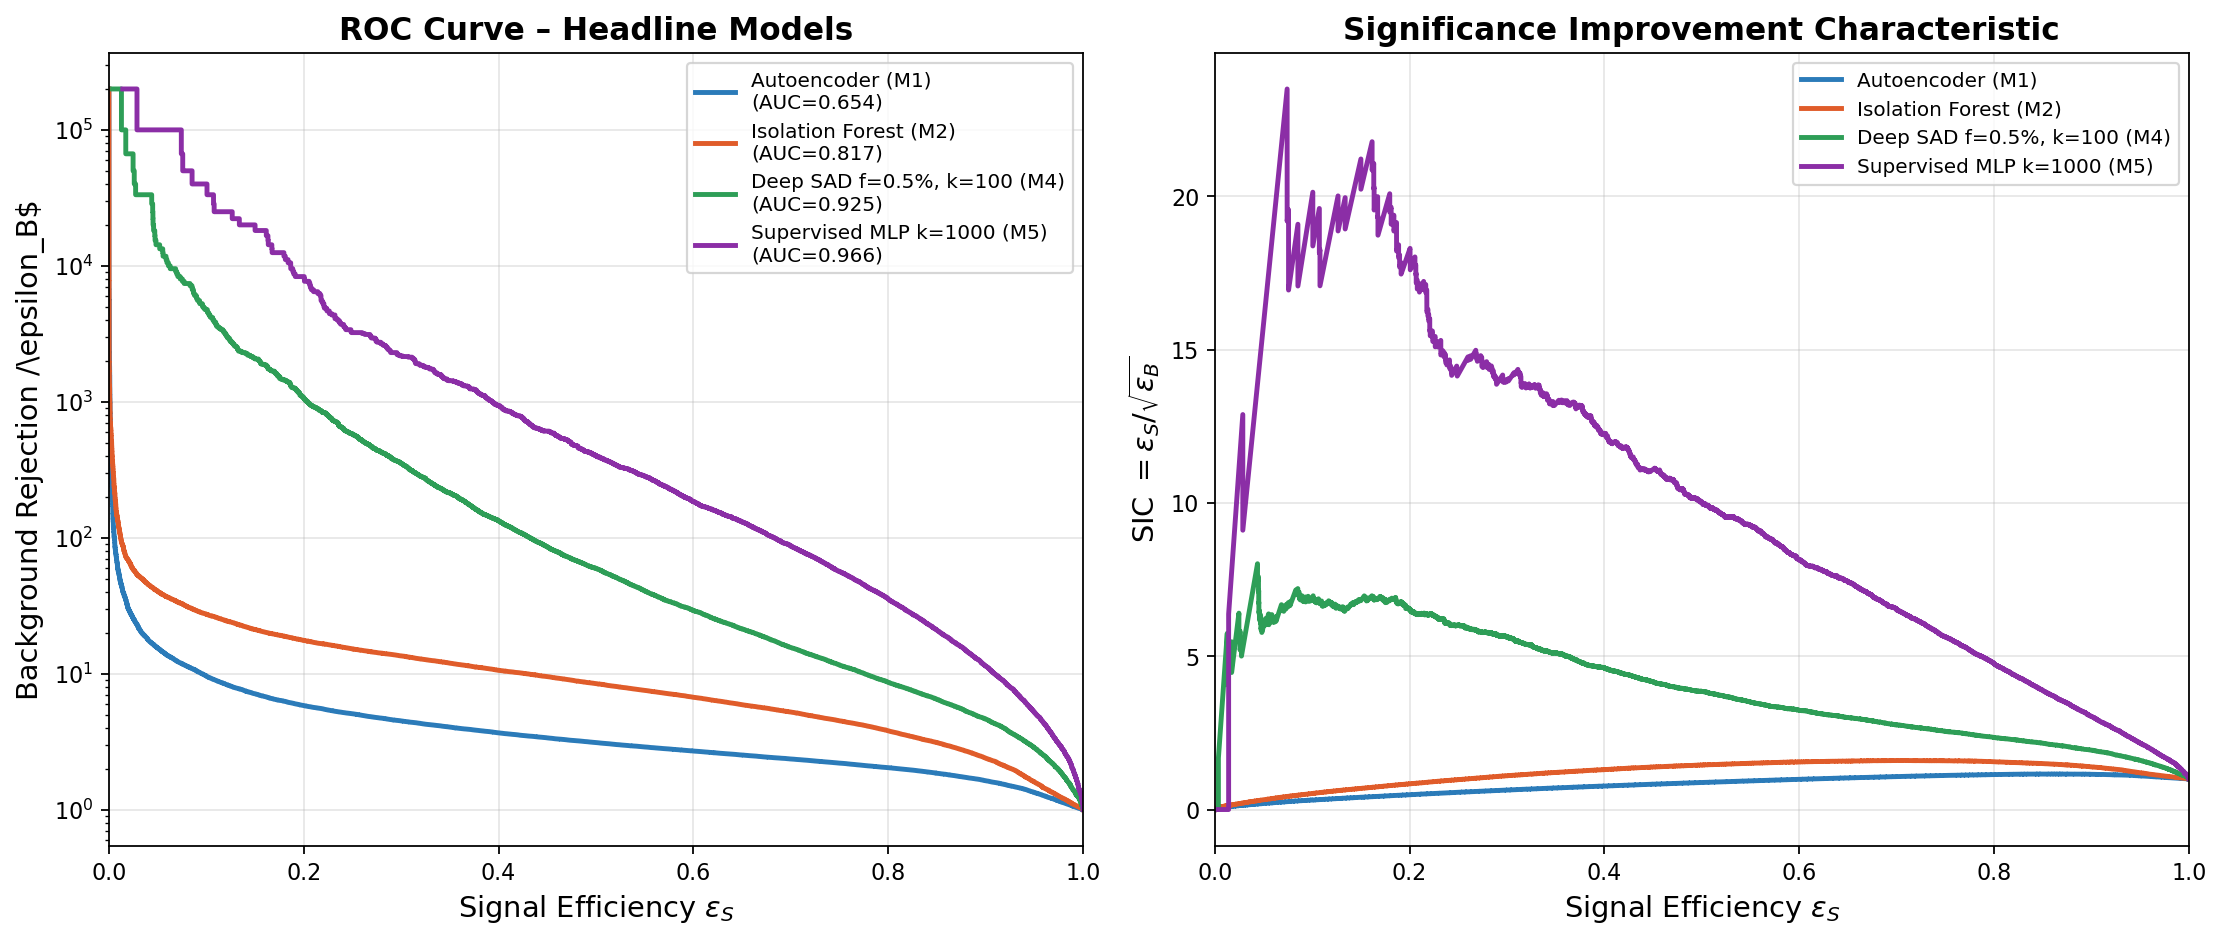
\includegraphics[width=0.94\textwidth]{headline_roc_sic_comparison.png}
\caption{Released seed-42 headline ROC curves and significance-improvement diagnostics. These single-seed curves supplement the five-seed AUC table; their counting approximation is not a discovery likelihood.}
\label{fig:roc}
\end{figure*}

\subsection{Contamination and known-anomaly budgets}
The single-seed contamination sweep is given in Table~\ref{tab:contamination}. The SVDD nominal AUC decreases from 0.5123 to 0.4439 between zero and 1\% contamination. Isolation Forest changes less across these four settings. These measurements do not establish monotonic population responses or causal mechanisms because most grid points lack repeated seeds and the sample of injected signal also changes.

\begin{table}[tbp]
\caption{Nominal AUC across the seed-42 unlabelled-contamination sweep. $f$ is expressed in percent of training background.}\label{tab:contamination}
\begin{ruledtabular}\begin{tabular}{rccc}
$f$ (\%) & Autoencoder & Isolation Forest & SVDD\\
0 & 0.7944 & 0.8165 & 0.5123\\
0.1 & 0.7035 & 0.8172 & 0.4866\\
0.5 & 0.7160 & 0.8179 & 0.4790\\
1 & 0.7240 & 0.8136 & 0.4439\\
\end{tabular}\end{ruledtabular}
\end{table}

\begin{table}[tbp]
\caption{Seed-42 Deep SAD nominal AUC as a function of contamination and number of known anomalies. The larger budget improves this grid's ranking; no optimal budget is inferred.}\label{tab:sadgrid}
\begin{ruledtabular}\begin{tabular}{rccc}
$f$ (\%) & $k=10$ & $k=100$ & $k=1000$\\
0 & 0.7611 & 0.8946 & 0.9282\\
0.5 & 0.8452 & 0.8762 & 0.9316\\
1 & 0.7695 & 0.8892 & 0.9258\\
\end{tabular}\end{ruledtabular}
\end{table}

In Table~\ref{tab:sadgrid}, the 1,000-label settings give AUCs near 0.93, while the 10-label settings vary substantially. The 100-label reference is a useful intermediate operating point, rather than a statistically demonstrated optimum. Because Eq.~\eqref{eq:sad} separately averages the labelled term within batches and omits it when no labels are present, a budget sweep changes both information and optimization dynamics. Controlled resampling and matched gradient exposure would be needed to separate these effects.

A descriptive way to summarize label efficiency is the fraction of the AUC gap from Isolation Forest to the fully supervised reference that the SAD headline closes:
\begin{equation}\label{eq:gapfraction}
 G_{\AUC}={\overline{\AUC}_{\mathrm{SAD}}-\overline{\AUC}_{\mathrm{IF}}\over
 \overline{\AUC}_{\mathrm{sup}}-\overline{\AUC}_{\mathrm{IF}}}=0.510.
\end{equation}
The current five-seed means therefore close approximately 51\% of this descriptive gap, rather than the approximately 80\% inferred from the historical draft. $G_{\AUC}$ is dimensionless and benchmark-dependent; it is neither a fraction of discoverable signals nor an efficiency per labelled event. It also inherits the preprocessing and validation differences of the supervised reference. No uncertainty interval for this ratio or universal label-budget optimum is claimed.

\subsection{Transfer and mass dependence}
The mean AUC falls by 0.1210 for the autoencoder, 0.1237 for Isolation Forest, and 0.1388 for Deep SAD when transferring from two-prong to three-prong signal. The fully supervised reference loses 0.0367. SVDD and the mass-aware variant instead increase to 0.6170 and 0.6670, respectively, from poor nominal rankings. These signed differences demonstrate topology dependence of the scores; an increase from a near-chance nominal result should not be presented as general-purpose anomaly sensitivity.

\begin{figure*}[tbp]
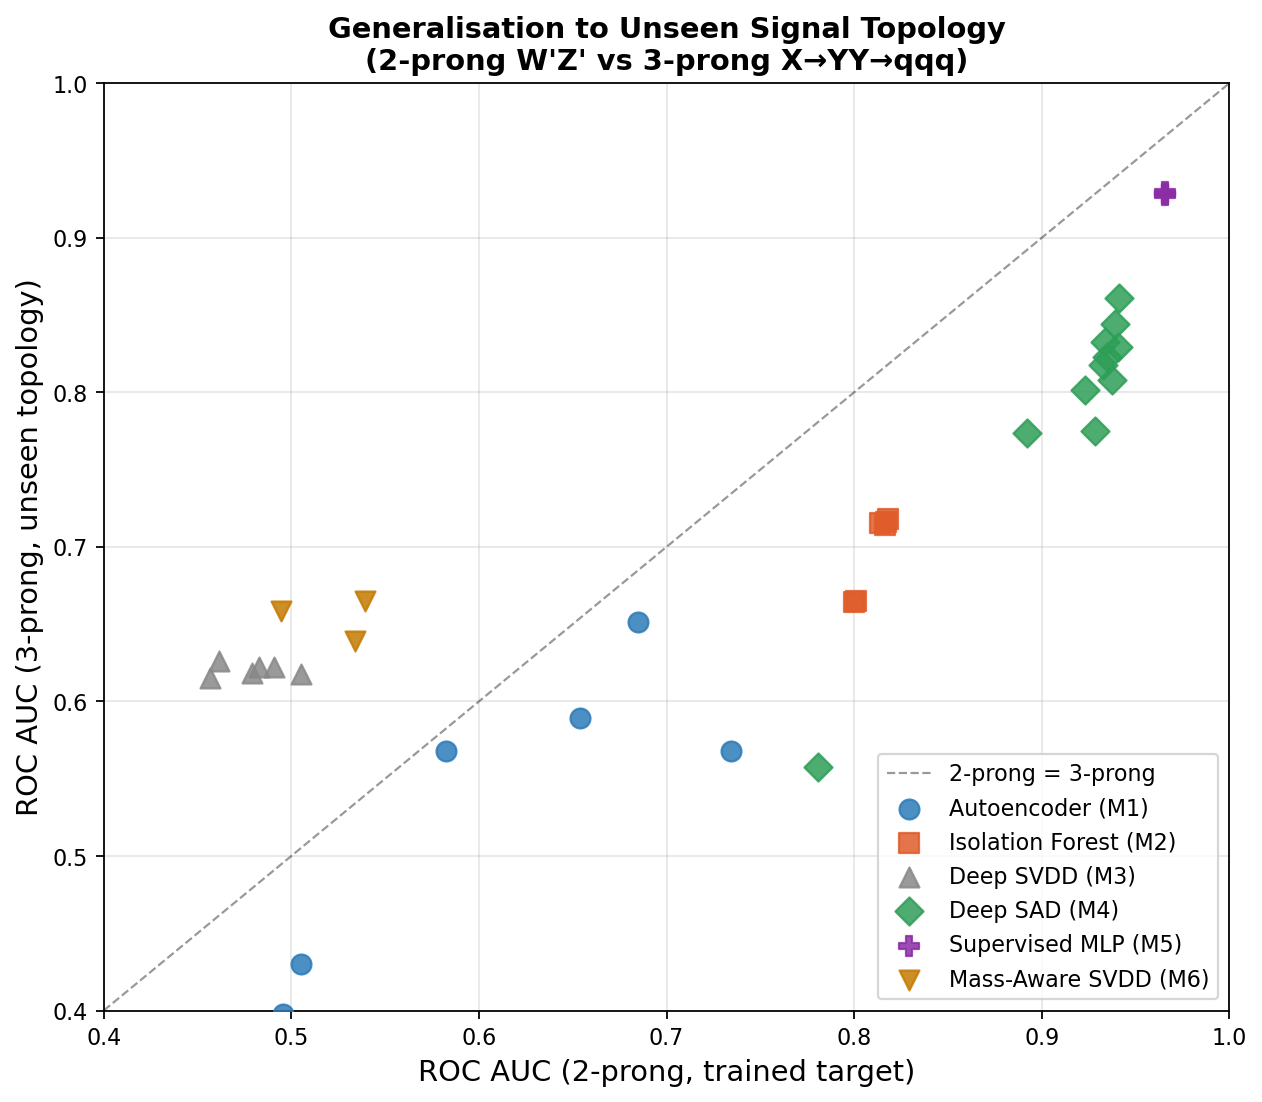
\includegraphics[width=0.46\textwidth]{generalisation_scatter.png}
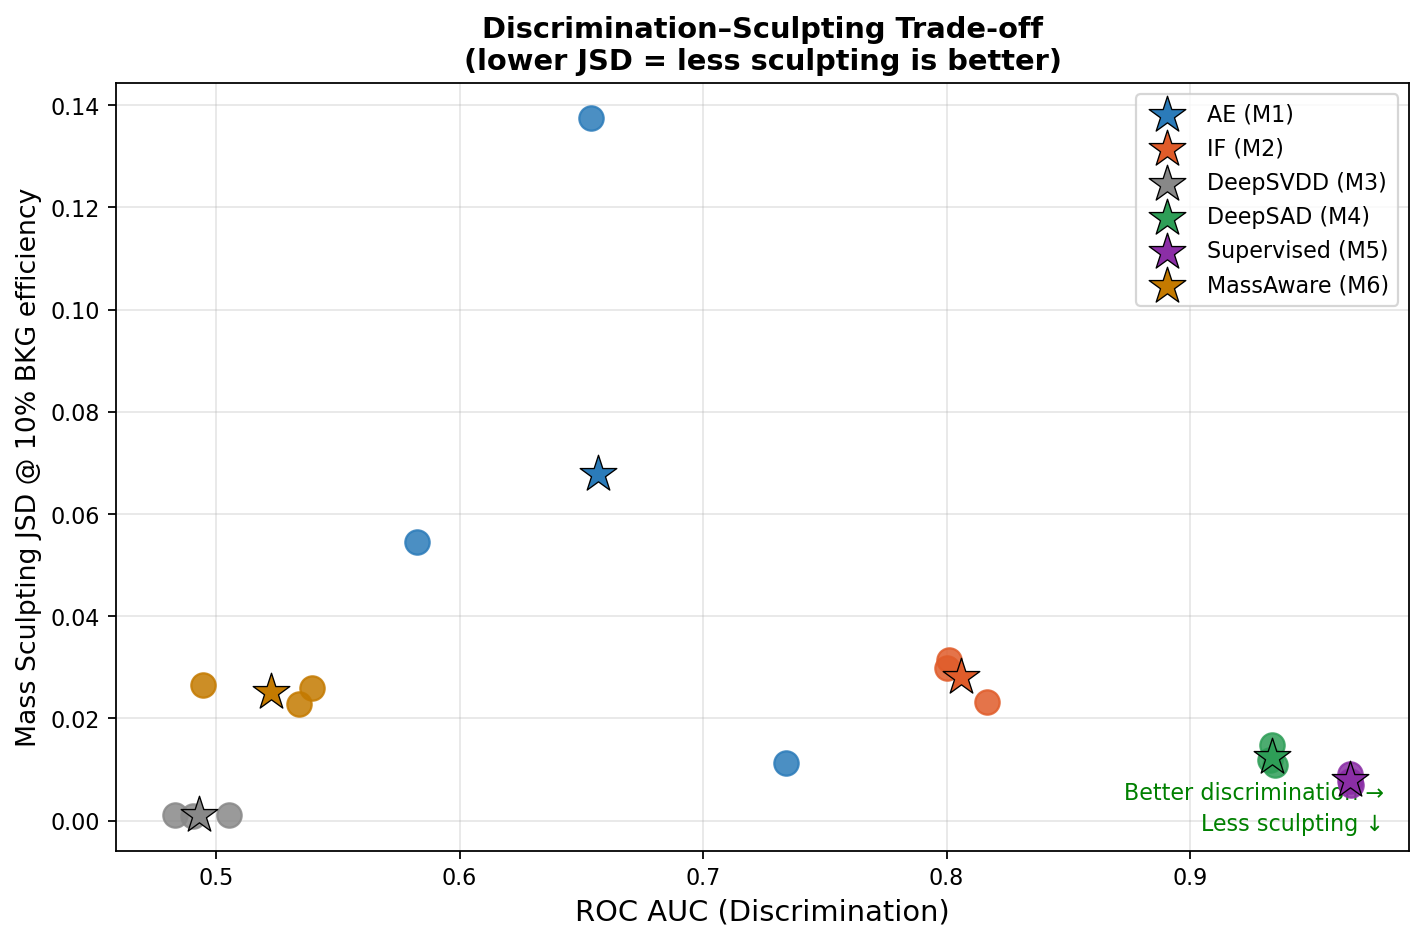
\includegraphics[width=0.46\textwidth]{jsd_vs_auc_tradeoff.png}
\caption{Released headline topology-transfer (left) and discrimination--mass-distortion (right) diagnostics. Dots show the five training seeds and stars their means for each headline setting in Table~\ref{tab:headline}. The mass comparison uses the 10\% background operating point. Binned JSD is a diagnostic, not a certificate of background-model adequacy.}
\label{fig:transfer}
\end{figure*}

Excluding $\mjj$ does not make a detector mass-independent: jet masses and substructure can be correlated with the event mass. The mean 10\% mass JSD is 0.0287 for Isolation Forest, 0.0066 for the Deep SAD headline, and 0.0082 for the supervised reference. The SVDD value 0.0012 accompanies near-chance nominal discrimination. Thus a small mass-histogram change is insufficient as a success criterion. Explicit mass inclusion in the specified SVDD reference yields JSD 0.0262 and nominal AUC 0.5151, without improving the nominal task.

The original study's mass diagnostics are retained in Fig.~\ref{fig:massprofiles}. Each frozen seed-42 panel compares inclusive and selected background mass spectra, mass-dependent background acceptance, and the score as a function of mass. These views complement the scalar JSD summary: a stable global histogram can conceal a narrow localized distortion, and a smooth change in acceptance can still alter the fitted sidebands. Features in a background-only spectrum cannot be explained by the injected signal, which is absent from that spectrum.

\begin{table*}[tbp]
\caption{Additional headline operating-point diagnostics, averaged over seeds 42--46. $R_a$ denotes background rejection at signal efficiency $a$\%; $\mathrm{SIC}_{\max}$ is the maximum finite-test significance-improvement characteristic. JSD$_{1\%}$ uses the frozen validation-background operating point, and $\rho$ is background score--mass Pearson correlation. These descriptive means have no claimed confidence intervals; the seed-42 maxima and test-ROC thresholds are not prospectively selected search cuts.}\label{tab:operating}
\begin{ruledtabular}\begin{tabular}{lrrrrrr}
Detector & $R_{10}$ & $R_{30}$ & $R_{50}$ & $\mathrm{SIC}_{\max}$ & JSD$_{1\%}$ & $\rho$\\
Autoencoder & 22.50 & 10.69 & 5.14 & 1.21 & 0.0292 & 0.0650\\
Isolation Forest & 28.97 & 13.08 & 7.76 & 1.52 & 0.0793 & 0.2846\\
Deep SVDD & 6.51 & 3.27 & 2.11 & 1.00 & 0.0082 & 0.0219\\
Deep SAD & 452.75 & 119.92 & 43.47 & 3.40 & 0.0178 & 0.0419\\
Supervised & 39330.19 & 2189.60 & 402.01 & 25.13 & 0.0123 & 0.0157\\
Mass-aware SVDD & 7.64 & 3.46 & 2.19 & 1.00 & 0.1087 & 0.0705\\
\end{tabular}\end{ruledtabular}
\end{table*}

Table~\ref{tab:operating} restores the original draft's distinction between a global ranking and a useful operating point. Ratios at small background rates can be sensitive to finite samples, and maximizing SIC on the test ROC is descriptive optimization over that sample. The table therefore complements the AUC uncertainty analysis rather than substituting for it or assigning discovery meaning to an ROC maximum.

\begin{figure*}[tbp]
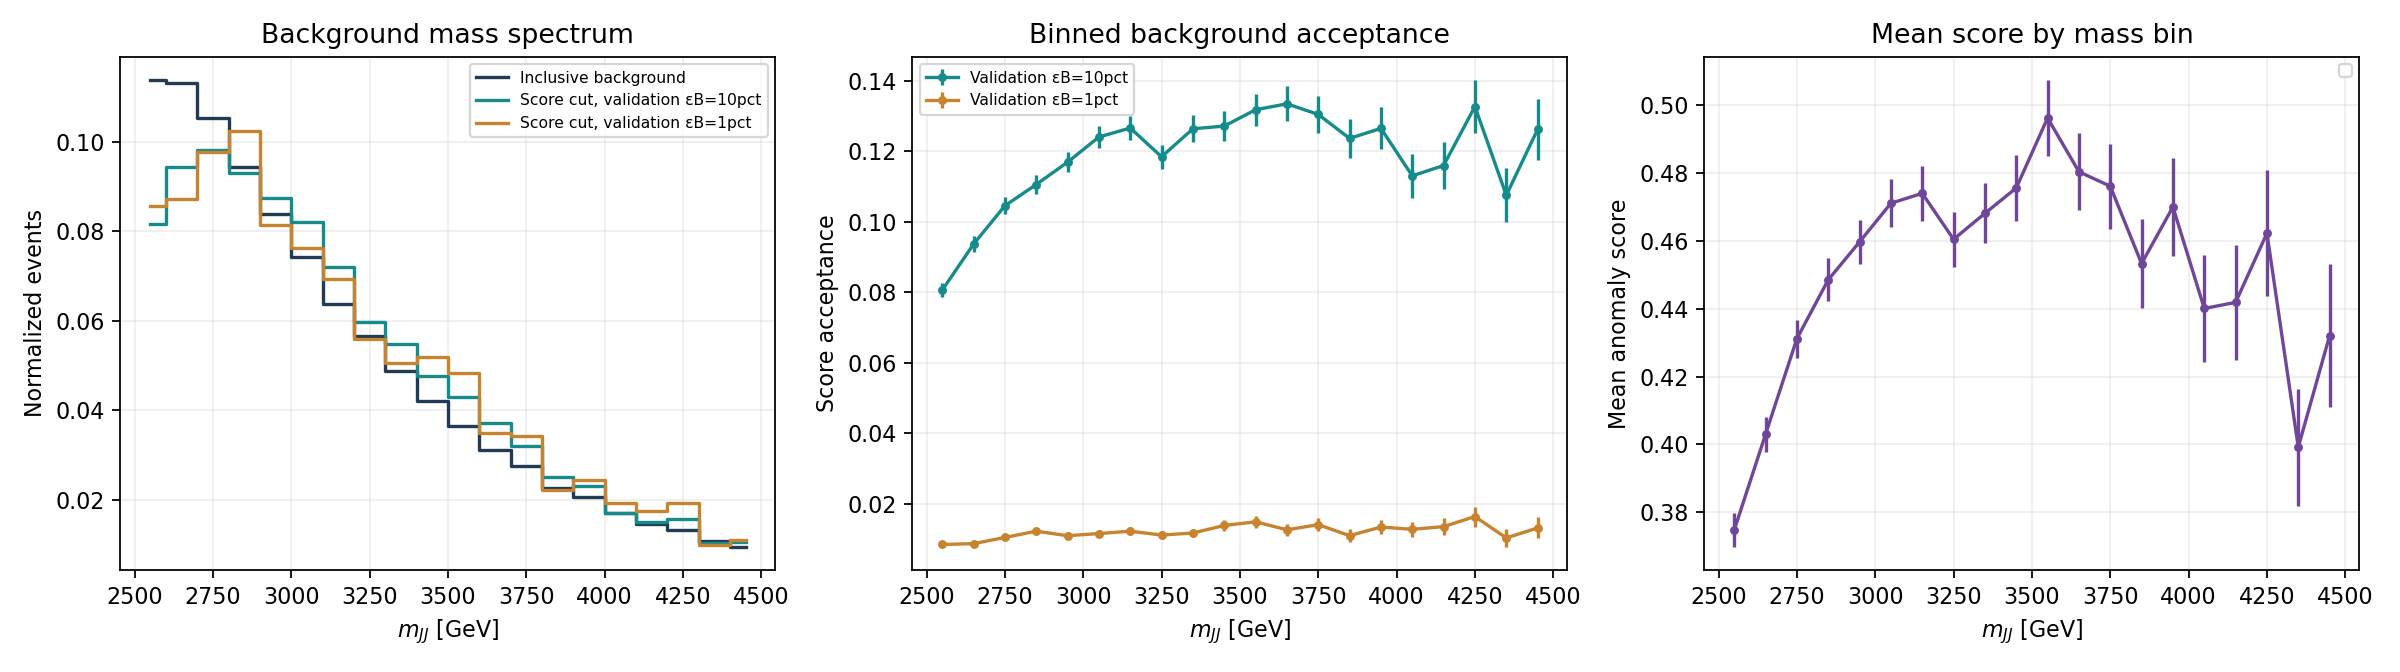
\includegraphics[width=0.95\textwidth]{M4_DeepSAD_f0.5_k100_42_mass_diagnostics.png}\\[3pt]
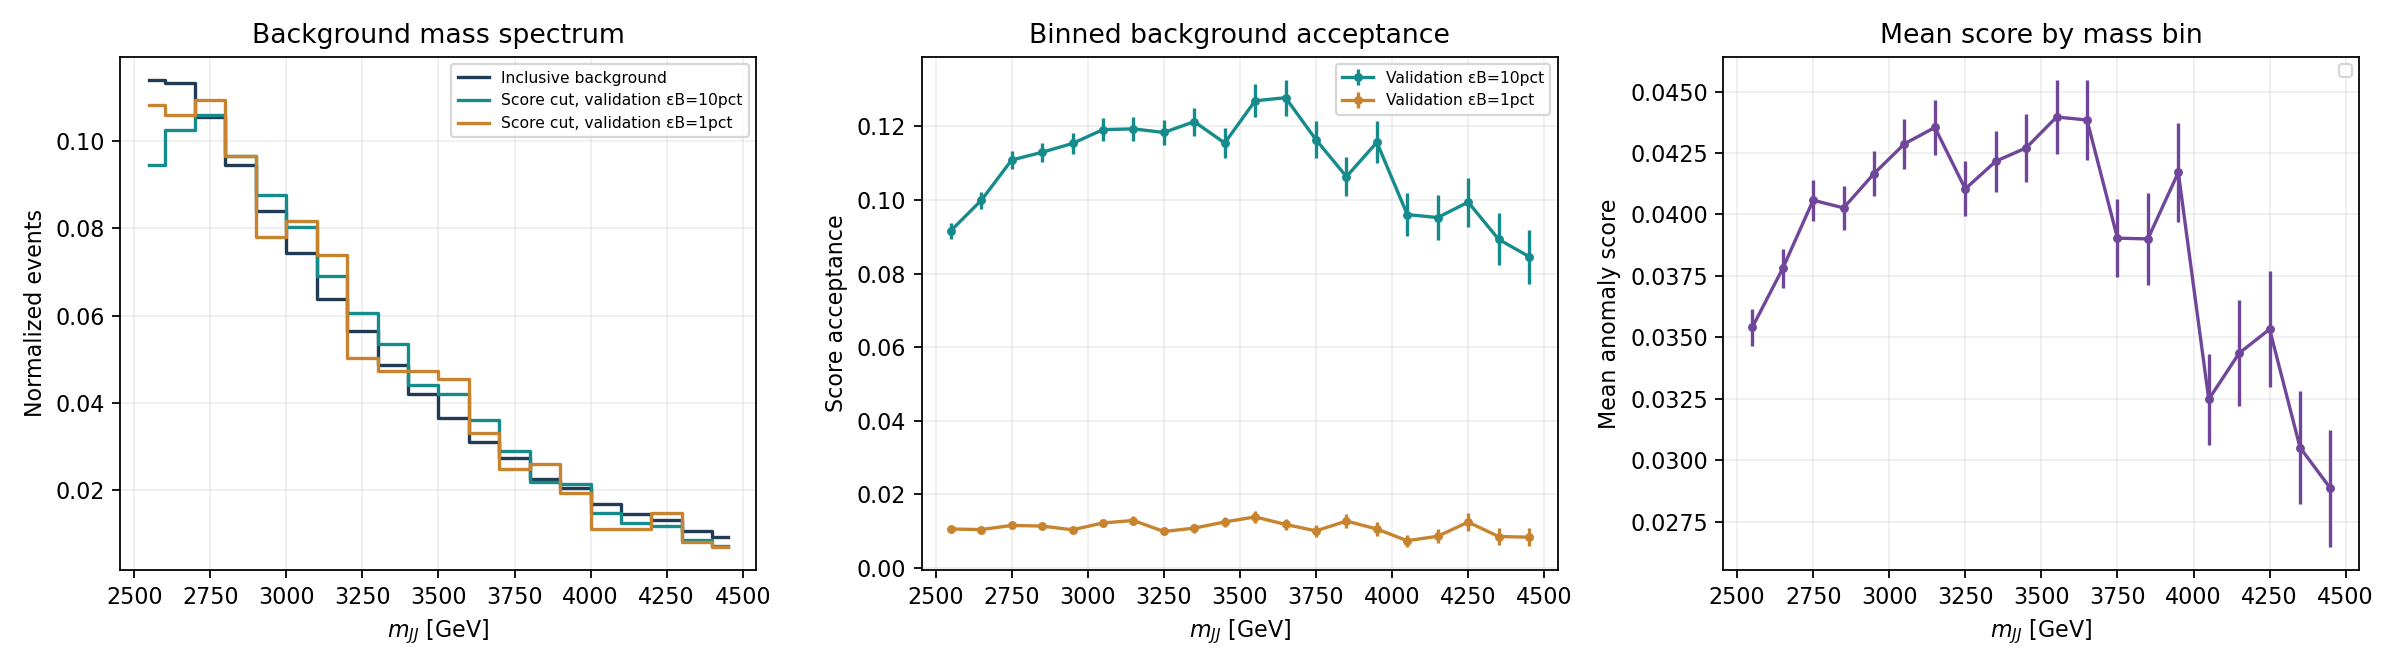
\includegraphics[width=0.95\textwidth]{M5_Supervised_f0_k1000_42_mass_diagnostics.png}
\caption{Background-only mass diagnostics for the Deep SAD headline (top) and supervised reference (bottom), seed 42. Within each row, the panels show mass distributions, bin-dependent acceptance, and score--mass dependence for the saved operating-point diagnostics. These plots are not signal-injection discovery tests.}\label{fig:massprofiles}
\end{figure*}

The sideband statistic can rise substantially after a cut. For example, at seed 42 the Deep SAD diagnostic gives $Z=5.89$ and $7.58$ at the 10\% and 1\% background operating points. The corresponding supervised values are $6.63$ and $13.69$. Table~\ref{tab:z} reports all five reference seeds, including the failed Deep SAD 1\% fit at seed 44. Omitting a failed fit from an average or a null distribution changes the estimand; these outputs cannot establish a reliable significance gain.

\section{Exploratory extensions}
The following results are archived, largely single-seed extensions. They were not part of the 47-fit clean core rerun and are not combined with its seed-dispersion estimates. Their purpose is to identify follow-up questions, not to enlarge the validated claim by counting heterogeneous experiments together.

\subsection{Particle-level reconstruction}
A background-only permutation-invariant autoencoder was trained for eight epochs on a seeded subset of 50,000 background training events and selected using all 199,984 validation background events. It uses masked particle encodings and mean/max pooling of up to 700 particle triples, followed by reconstruction of valid particle features. The inputs encode normalized transverse momentum, its logarithmic transforms, pseudorapidity, and sine/cosine of azimuth. The logarithm of $1+p_T$ in the numerical implementation assumes $p_T$ measured in GeV; its dimensionally explicit interpretation is $\ln(1+p_T/(1\,\mathrm{GeV}))$. No signal training labels are used in this extension.

Nominal AUC is 0.4980 on the core test background and signal events, while the raw three-prong sample gives 0.4409. The latter uses all 100,000 raw events, rather than the 99,975-event high-level validity-filtered pool. At a frozen 1\% validation-background threshold the nominal and three-prong signal efficiencies are 0.160\% and 0.098\%. On the additional public $X\to YY'\to4q$ and $W_{KK}\to WR\to3W$ samples \cite{external}, evaluated against a fixed 20,000-event background subset, AUCs are 0.4647 and 0.5068; signal efficiencies at that same threshold are 0.159\% and 0.280\%, respectively. The two signal pools contain 44,673 and 32,801 events and use a different generation chain from the original benchmark. These sample-specific negative results do not demonstrate absence of useful particle-level information. Architecture, reconstruction target, training duration, and transfer of the reference distribution remain untested explanations.

Semi-supervised permutation-invariant collider detectors already exist \cite{antelope}, and recent work studies optimal-transport event representations \cite{ot}. The present small reconstruction experiment neither reproduces those approaches nor establishes a new general limitation of constituent representations.

\subsection{Density proxies and calibration}
The archived ``ANODE''-named configuration is a five-component Gaussian mixture fitted to background sidebands, with negative log background density as its score. It does not estimate the signal-region data density, form an ANODE likelihood ratio, or implement mass-conditional interpolation. Likewise the ``CATHODE''-named conditional variational-autoencoder extension is a generated-reference classifier proxy, rather than the published conditional-flow construction \cite{anode,cathode}. Their observed AUCs, approximately 0.720 and 0.481, cannot be used to infer the performance of the original methods.

The archived region MLP and region-tree classifiers give nominal AUCs of approximately 0.605 and 0.575. Both classifier implementations use only the first five feature columns at prediction time; $\mjj$ defines their training-region labels rather than entering their predictor directly. Their archived $f=0$ settings contain background only during training, so a signal-enriched training mixture is not present. They can learn background differences between regions without thereby learning the nominal signal. Their ranking is an observation about these settings, not evidence against weakly supervised mixture classification \cite{cwola}.

For the frozen mixture score, the held-out sideband pool contains 128,112 events, split equally into calibration and evaluation sets using seed 2026. The conformal tail value is
\begin{equation}\label{eq:conformal}
 p(x)={1+\sum_{i=1}^{n_{\mathrm{cal}}}\mathbf1[s_i\geq s(x)]\over n_{\mathrm{cal}}+1}.
\end{equation}
Under exchangeability of calibration and future background scores and a fixed scoring model, this standard rank construction is conservative at finite sample size \cite{conformal}. The measured evaluation rejection rates are 1.054\%, 4.975\%, and 9.868\% at nominal 1\%, 5\%, and 10\% levels. The reported uniformity diagnostic has a Kolmogorov--Smirnov statistic of 0.0043 and nominal $p=0.179$; common calibration events and discrete ranks mean this diagnostic is not a stand-alone proof of uniform independent draws. The exercise checks same-sideband score calibration, not background-density correctness or transfer into a signal region. Recent collider work explicitly addresses conformal calibration, mass sculpting, and look-elsewhere effects \cite{araz}; Eq.~\eqref{eq:conformal} itself is not a novel contribution here.

\section{Discussion and limitations}
The strongest supported empirical conclusion is that a modest set of known anomalies improves the specified hypersphere detector's nominal ranking in this benchmark, while sensitivity to a changed topology and mass distortion remain separate concerns. That conclusion is consistent with the existing purpose of Deep SAD \cite{sad}; it establishes an implementation-specific measurement, not a new learning principle. The negative SVDD and particle-level results are reproducible observations with unresolved causes.

\subsection{Practical interpretation of the four questions}
The contamination sweep gives Isolation Forest the most stable nominal ranking among the three learned unsupervised implementations tested at seed 42, while the autoencoder's seed dispersion cautions against interpreting a single fit. Limited supervision raises the SAD ranking, but its approximately 51\% gap closure and the changed topology distinguish useful label guidance from an approximation to a universal signal model. The mass comparison identifies a second requirement: a ranking improvement must be assessed alongside how the selection changes the background that a resonance search will fit. Finally, the held-out three-prong pool measures one concrete transfer task, rather than broad model independence.

These observations support a joint reporting standard: identify the supervision resource, give the contamination convention and seeds, report the nominal and transferred rankings, and show background-shape diagnostics at validation-defined thresholds. A detector with a slightly lower global AUC may be preferable for a particular search if its relevant operating point and background model are better controlled; the present study does not supply the full likelihood and systematic uncertainties needed to make that deployment choice. Likewise, removing a mass input or adding a decorrelation penalty is a design constraint, not a certificate of valid inference \cite{disco}.

\subsection{Failure diagnostics and label bookkeeping}
The original draft correctly emphasized that implementation failures can resemble physical conclusions. The current evidence establishes near-chance nominal SVDD ranking, but does not justify the stronger historical claim that center, activation, bias, and depth ablations demonstrated a universal collapse mechanism. Appendix~\ref{app:diagnostics} gives a restricted linear example to clarify what a constant-score limit would imply and why it does not diagnose the actual nonlinear model. Latent variance, score variance, gradient norms, and comparisons with pretrained embeddings would be needed to connect that example to the observed runs.

For Deep SAD, unlabelled contamination and known anomalies must remain separate. If every injected signal were accidentally labelled, a nominal contamination sweep would simultaneously increase supervision and change its scientific meaning. In the released implementation only the designated $k$ events enter the anomalous-label term; injected but unlabelled events enter the reference term. Event-index disjointness and label-isolation checks are therefore part of the evidence, rather than optional bookkeeping. Historical performance differences cannot be assigned to that possible failure mode without a run-specific provenance comparison.

\subsection{Mass-decorrelated and extended-feature research directions}
The original MD-SWAD idea is retained as a concrete candidate in Appendix~\ref{app:mdswad}. Matching a spread-out reference distribution and penalizing mass dependence targets limitations different from those of a point-centered hypersphere. However, the previous draft's M9/M10 AUC and mass-decorrelation numbers do not have matching validated evaluation tables in the current release; they are not restored as experimental findings. The sliced-Wasserstein and distance-correlation ingredients already have prior art \cite{sliced,disco}. The scientific question is whether their particular combination gives a reproducible advantage under a matched collider protocol, not whether its name alone establishes novelty.

The seven-feature extension similarly preserves a useful hypothesis from the draft: $\tau_{32}=\tau_3/\tau_2$ can expose substructure information beyond $\tau_{21}$ \cite{tau}. Its ability to improve the held-out ranking depends on the signal/background distributions, the reference training objective, and consistent feature extraction. The inequality $\tau_{32}<1$ alone is not a discriminating rule against QCD. Appendix~\ref{app:extended} states the corrected column schema and the validation needed before an improvement claim.

Several limitations constrain generalization. First, the same fixed simulated test events are used across seeds and configurations. The bootstrap intervals quantify sampling uncertainty conditional on these distributions, not detector response, hadronization, or unseen resonance masses. Second, only six configurations have five-seed coverage, and no prospective hyperparameter selection or independent final holdout is claimed. Third, the supervised scaler and validation objective differ from those of the other models, while label exposure in Deep SAD changes with minibatch composition. Fourth, a physics-motivated cut and faithful modern density/particle baselines require matched-protocol comparisons before a claim of competitive novelty.

The significance diagnostic is especially limited. Bounded sideband fits require at least six positive bins, numerical convergence, and a fitted total sideband yield within a factor two of the observed yield. Fifty background-only Poisson bootstrap trials per core configuration are too few to resolve a rare discovery tail. An older 500-trial closure exercise for the autoencoder, Isolation Forest, and the conditional-generator proxy retained 461, 479, and 456 valid fits, respectively, at the 1\% background cut after failures. These archived checks concern older checkpoints, and conditioning on fit survival can distort a null distribution. Neither a small observed false-positive fraction nor a large approximate $Z$ validates final-model discovery inference. A future study must define outcomes for failed fits, calibrate the complete procedure, and account for selection and any mass scan.

The clean core reproduction demonstrates executability, but not bitwise portability of every neural result. Historical and fresh results differ by as much as about 0.211 in autoencoder AUC and 0.171 in Deep SAD AUC at overlapping configurations, whereas some other reference scores agree. The release makes the fresh environment and outputs canonical; the causes of the neural differences have not been isolated in a factorial environment or optimization study. It would be unjustified to attribute them solely to a particular thread setting or library version.

Finally, a public benchmark with one principal family of simulated signals cannot establish a discovery on experimental data. The exploratory evaluations of additional hypotheses are too limited to replace a prospectively defined, multi-hypothesis validation campaign.

\section{Conclusions}
We provide an audited comparison of six reference detectors and a limited contamination/label-budget grid on a common LHC Olympics feature representation. Five-seed results show useful nominal discrimination for Isolation Forest, stronger ranking for a Deep SAD configuration using 100 known anomalies, and the largest AUC for a fully supervised reference. Finite-test paired bootstrapping confirms the seed-42 ranking differences within its conditional scope. A three-prong evaluation exposes topology sensitivity, while mass diagnostics show that good ranking and benign background shapes cannot be inferred from each other.

The released evidence supports an empirical technical study with transparent negative results and reproducibility artifacts. It does not establish a new anomaly-detection algorithm, a state-of-the-art comparison, or a calibrated discovery significance. The next scientific step is a focused mechanism study with matched preprocessing and strong baselines, prospectively fixed evaluation on additional hypotheses, and a statistically valid treatment of the full background-selection and sideband-fit procedure.

\section*{Data and code availability}
The dataset is publicly available through Zenodo \cite{dataset}. The code and core result artifacts are available at \url{https://github.com/lihtim-kitsa/lhc-olympics-2020}, release v1.0.1, commit \texttt{4b15306cfac9e3f57ace098932db0e4ea69e0f2a}. Canonical tables, frozen scores, bootstrap intervals, and environment specifications accompany that release. The manuscript and its data audit are subsequent documentation artifacts; the release identifier refers to the numerical core, not to a newly tagged manuscript version. Raw datasets and local checkpoints are not all embedded in Git and require the documented retrieval/reproduction steps.

\section*{Acknowledgments and AI-use disclosure}
Author and affiliation details are retained from the existing project manuscript. Funding and contribution statements must be confirmed by the responsible researcher before submission. OpenAI Codex (GPT-6; session of October 3, 2026) assisted with repository auditing, manuscript drafting, literature retrieval, interpretation checks, and document preparation. Numerical statements were checked against saved project artifacts, and cited literature was checked against primary records. This assistance does not replace independent author review of the scientific argument, citations, statistical assumptions, or final text; that review remains necessary before submission. No AI system is listed as an author.

\appendix
\section{Local-fit outputs and reproducibility details}
\begin{table}[tbp]
\caption{Approximate local-excess diagnostic of Eq.~\eqref{eq:z} after nominal validation-background cuts. ``Failed'' is retained explicitly. Values are not calibrated discovery significances.}\label{tab:z}
\begin{ruledtabular}\begin{tabular}{lrrr}
Detector & Seed & 10\% cut & 1\% cut\\
Deep SAD & 42 & 5.89 & 7.58\\
Deep SAD & 43 & 4.71 & 5.80\\
Deep SAD & 44 & 4.13 & Failed\\
Deep SAD & 45 & 4.95 & 7.51\\
Deep SAD & 46 & 4.87 & 8.43\\
Supervised & 42 & 6.63 & 13.69\\
Supervised & 43 & 6.66 & 14.71\\
Supervised & 44 & 7.76 & 14.86\\
Supervised & 45 & 6.59 & 13.76\\
Supervised & 46 & 6.32 & 13.96\\
\end{tabular}\end{ruledtabular}
\end{table}

The shape-fit bounds are $a\in[-50,50]$, $b,c\in[-20,60]$, and $d\in[-20,20]$, with a log-count regression initializer and L-BFGS-B optimization. Fisher-matrix inversion uses a pseudoinverse with tolerance $10^{-12}$. These numerical choices are part of the diagnostic procedure and can affect low-count or boundary fits. A joint likelihood with robust background-model uncertainty and integer randomized event acceptance, or an explicitly calibrated weighted-data treatment, is required for a stronger inference.

The final core used an isolated Python 3.11.9 environment on Windows, with NumPy 2.3.5, pandas 2.3.3, scikit-learn 1.7.2, SciPy 1.16.3, h5py 3.15.1, and CPU PyTorch 2.13.0. The dependency lock additionally records hdf5plugin 6.0.0 and FastJet 3.5.1.5. A fresh checkout rebuilt feature/split artifacts and reran all 47 core fits using shared checksum-verified raw data, isolated output stores, and one PyTorch thread per worker. The staged run took approximately 33.3 minutes including pauses and excluding data retrieval; this is a machine-specific observation, not a universal runtime guarantee. Raw input storage was about 3.223 GB, with approximately 61.6 MB of cached features, 10.5 MB of model artifacts, and 11.5 MB of figures, excluding environments and worker duplication. Peak memory was not measured.

Thirty repository tests passed in the release verification. These include split/scaler isolation, labelled/unlabelled disjointness, threshold ties, and AUC bootstrap consistency; software tests do not establish physics validity. The accompanying data audit derives the manuscript's numerical tables from the canonical results without fitting new models. An independent cross-machine reproduction and human scientific review remain outstanding.

\section{An illustrative constant-score limit}\label{app:diagnostics}
Consider the restricted linear embedding $\phi_W(x)=Wx$ with fixed center $c$, no bias, finite second moments, and an exactly centered training reference $\mu=\mathbb E[x]=0$. Writing $\Sigma=\mathbb E[xx^T]$, its squared-distance objective is
\begin{align}
 L(W)&=\mathbb E\|Wx-c\|^2\\
 &=\operatorname{tr}(W\Sigma W^T)-2c^TW\mu+\|c\|^2,\\
 \nabla_W L&=2W\Sigma-2c\mu^T.
\end{align}
At $\mu=0$, $W=0$ is stationary and minimizes this linear objective; if $\Sigma$ is positive definite, it is the unique minimum. The score then becomes $s(x)=\|c\|^2$ for every event, giving AUC $1/2$ under half-credit tie handling. All terms are dimensionless for standardized inputs, and the $c=0$ limit gives the expected zero score.

This calculation illustrates a failure mode of a linear point-concentration objective, consistent with the motivation for architectural restrictions in Deep SVDD \cite{svdd}. It is not a derivation for the trained multilayer ReLU network: centering $x$ does not imply centering $\phi_\theta(x)$ or the parameter Jacobian, and the center in this project is initialized from embeddings rather than set identically to $0.1\mathbf1$. Near-chance AUC can also occur with varying scores that fail to separate the evaluated classes. Diagnosing collapse requires inspecting the learned representation rather than inferring it from AUC alone.

\section{Mass-decorrelated sliced-Wasserstein candidate}\label{app:mdswad}
Let $z_i=\phi_\theta(x_i)\in\mathbb R^{16}$ denote an embedding of an unlabelled batch of size $n$. Draw $n$ reference vectors $\xi_i\sim\mathcal N(0,I)$ and $K=50$ random unit directions $u_k$. The implemented empirical sliced squared-Wasserstein term is
\begin{equation}
 \widehat{\mathrm{SW}}_2^2={1\over Kn}\sum_{k=1}^K\sum_{i=1}^n
 \left[(u_k^Tz)_{(i)}-(u_k^T\xi)_{(i)}\right]^2,
\end{equation}
where $(i)$ denotes the sorted projected sample, not an event pairing. The construction follows the established use of one-dimensional transport along random projections \cite{sliced}. Reference vectors and projections are resampled in the implementation.

The candidate training loss is
\begin{equation}\label{eq:mdswad}
 L_{\mathrm{MD}}=\widehat{\mathrm{SW}}_2^2+
 \lambda\,\widehat{\mathrm{dCor}}(z,\mjj).
\end{equation}
The repository uses distance correlation itself, whereas the original draft wrote its square. Distance correlation is computed from doubly centered pairwise distance matrices and is dimensionless; the standard-normal latent coordinates make the transport term dimensionless as well. The mass variable enters the regularizer, not the anomaly-score input. Using finite-batch penalties does not demonstrate population independence \cite{disco}. Unlike the core bias-free SVDD backbone, this candidate's linear layers have biases.

For the labelled-anomaly variant, the implementation adds
\begin{equation}
 {\eta\over k}\sum_{j\in A}{1\over\|\phi_\theta(x_j)\|^2+10^{-6}},
 \qquad \eta=1,
\end{equation}
and evaluates the entire designated label pool at each unlabelled update. This exposure differs from the sparse mixed-batch Deep SAD schedule, so a direct label-efficiency comparison must account for it. The anomaly score is $\|z\|^2$, which would be monotonic in negative log density for an exactly standard-normal embedding. Neither exact distribution matching nor a calibrated Gaussian tail has been established for the trained candidate.

Equations above document an implemented research direction, not a validated solution to collapse or mass sculpting. Required tests include transport-only and decorrelation-only ablations, a prospectively selected $\lambda$, matched label exposure, repeated seeds, and background-only search calibration. The candidate's historical numerical table is withheld until checkpoint, feature schema, and evaluation provenance match.

\section{Extended subjettiness representation}\label{app:extended}
The corrected extended cache has schema version 2.0.0 and ordered columns
\begin{align*}
 (&m_{J_1},|\Delta m_J|,\tau_{21}^{J_1},\tau_{21}^{J_2},\Delta R_{JJ},\\
  &\tau_{32}^{J_1},\tau_{32}^{J_2},\mjj,y).
\end{align*}
Its first five columns preserve the canonical input ordering. A previous cache placed $\Delta R_{JJ}$ after the additional ratios, so reusing positional slices could silently change the detector's inputs. Schema and column checks prevent that mismatch; they do not establish improved discrimination. Finite, well-defined ratios and identical event selections must also be enforced before comparing a seven-feature fit with its five-feature reference.

The feature extension is motivated by the three-prong evaluation and established subjettiness observables \cite{tau}, but no validated repeated-seed result is used here to claim a gain. A suitable comparison would hold the split, training information, score orientation, and model-selection protocol fixed, then assess the new topology alongside the nominal task and mass diagnostics. The raw-particle exploratory results use a different representation and therefore do not serve as that ablation.

\begin{thebibliography}{99}
\bibitem{lhco} G. Kasieczka \textit{et al.}, The LHC Olympics 2020: A community challenge for anomaly detection in high energy physics, Rep. Prog. Phys. \textbf{84}, 124201 (2021), \href{https://doi.org/10.1088/1361-6633/ac36b9}{doi:10.1088/1361-6633/ac36b9}, arXiv:2101.08320.
\bibitem{dataset} G. Kasieczka, B. Nachman, and D. Shih, LHC Olympics 2020 R\&D Dataset, Zenodo (2019; version 5, 2022), \href{https://doi.org/10.5281/zenodo.6466204}{doi:10.5281/zenodo.6466204}.
\bibitem{svdd} L. Ruff \textit{et al.}, Deep one-class classification, in \textit{Proceedings of ICML}, Proc. Mach. Learn. Res. \textbf{80}, 4393 (2018), \url{https://proceedings.mlr.press/v80/ruff18a.html}.
\bibitem{sad} L. Ruff \textit{et al.}, Deep semi-supervised anomaly detection, in \textit{Proceedings of ICLR} (2020), \href{https://arxiv.org/abs/1906.02694}{arXiv:1906.02694}.
\bibitem{cwola} J. H. Collins, K. Howe, and B. Nachman, Anomaly detection for resonant new physics with machine learning, Phys. Rev. Lett. \textbf{121}, 241803 (2018), \href{https://doi.org/10.1103/PhysRevLett.121.241803}{doi:10.1103/PhysRevLett.121.241803}.
\bibitem{anode} B. Nachman and D. Shih, Anomaly detection with density estimation, Phys. Rev. D \textbf{101}, 075042 (2020), \href{https://doi.org/10.1103/PhysRevD.101.075042}{doi:10.1103/PhysRevD.101.075042}.
\bibitem{cathode} A. Hallin \textit{et al.}, Classifying anomalies through outer density estimation (CATHODE), Phys. Rev. D \textbf{106}, 055006 (2022), \href{https://doi.org/10.1103/PhysRevD.106.055006}{doi:10.1103/PhysRevD.106.055006}.
\bibitem{tau} J. Thaler and K. Van Tilburg, Identifying boosted objects with N-subjettiness, J. High Energy Phys. \textbf{03} (2011) 015, \href{https://doi.org/10.1007/JHEP03(2011)015}{doi:10.1007/JHEP03(2011)015}.
\bibitem{autoencoder} M. Farina, Y. Nakai, and D. Shih, Searching for new physics with deep autoencoders, Phys. Rev. D \textbf{101}, 075021 (2020), \href{https://doi.org/10.1103/PhysRevD.101.075021}{doi:10.1103/PhysRevD.101.075021}.
\bibitem{iforest} F. T. Liu, K. M. Ting, and Z.-H. Zhou, Isolation forest, in \textit{Proceedings of ICDM} (2008), pp. 413--422, \href{https://doi.org/10.1109/ICDM.2008.17}{doi:10.1109/ICDM.2008.17}.
\bibitem{cowan} G. Cowan, K. Cranmer, E. Gross, and O. Vitells, Asymptotic formulae for likelihood-based tests of new physics, Eur. Phys. J. C \textbf{71}, 1554 (2011), \href{https://doi.org/10.1140/epjc/s10052-011-1554-0}{doi:10.1140/epjc/s10052-011-1554-0}.
\bibitem{antelope} G. Matos, E. Busch, K. R. Park, and J. Gonski, Semi-supervised permutation invariant particle-level anomaly detection, J. High Energy Phys. \textbf{05} (2025) 116, \href{https://doi.org/10.1007/JHEP05(2025)116}{doi:10.1007/JHEP05(2025)116}, arXiv:2408.17409.
\bibitem{ot} T. Cai, A. Bhargava, and B. Nachman, Optimal transport event representation for anomaly detection, Phys. Rev. D \textbf{114}, 016011 (2026), \href{https://doi.org/10.1103/wwzk-25sy}{doi:10.1103/wwzk-25sy}, arXiv:2512.04839.
\bibitem{external} R. Das \textit{et al.}, Additional signal models for the LHCO2020 R\&D, Zenodo (2026), \href{https://doi.org/10.5281/zenodo.18983506}{doi:10.5281/zenodo.18983506}.
\bibitem{conformal} G. Shafer and V. Vovk, A tutorial on conformal prediction, J. Mach. Learn. Res. \textbf{9}, 371 (2008), \href{https://arxiv.org/abs/0706.3188}{arXiv:0706.3188}.
\bibitem{araz} J. Y. Araz and M. Spannowsky, Conformal calibration and look-elsewhere effect in anomaly detection for new-physics searches, \href{https://arxiv.org/abs/2606.13780}{arXiv:2606.13780} (2026), preprint.
\bibitem{atlas} G. Aad \textit{et al.} (ATLAS Collaboration), Dijet resonance search with weak supervision using $\sqrt{s}=13$ TeV collisions in the ATLAS detector, Phys. Rev. Lett. \textbf{125}, 131801 (2020), \href{https://doi.org/10.1103/PhysRevLett.125.131801}{doi:10.1103/PhysRevLett.125.131801}.
\bibitem{cms} V. Chekhovsky \textit{et al.} (CMS Collaboration), Model-agnostic search for dijet resonances with anomalous jet substructure in proton--proton collisions at $\sqrt{s}=13$ TeV, Rep. Prog. Phys. \textbf{88}, 067802 (2025), \href{https://doi.org/10.1088/1361-6633/add762}{doi:10.1088/1361-6633/add762}, arXiv:2412.03747.
\bibitem{disco} G. Kasieczka and D. Shih, DisCo Fever: Robust networks through distance correlation, Phys. Rev. Lett. \textbf{125}, 122001 (2020), \href{https://doi.org/10.1103/PhysRevLett.125.122001}{doi:10.1103/PhysRevLett.125.122001}, arXiv:2001.05310.
\bibitem{sliced} N. Bonneel, J. Rabin, G. Peyr\'e, and H. Pfister, Sliced and Radon Wasserstein barycenters of measures, J. Math. Imaging Vis. \textbf{51}, 22--45 (2015), \href{https://doi.org/10.1007/s10851-014-0506-3}{doi:10.1007/s10851-014-0506-3}.
\end{thebibliography}
\end{document}
